\documentclass[../Cover.tex]{subfiles}

\begin{document}

	\begin{minipage}[t][0.2\textheight][t]{0.1\textwidth} 
		\includegraphics[width=\textwidth]{\logoname}
	\end{minipage}
	\hfill
	\begin{minipage}[t][0.2\textheight][t]{0.8\textwidth}
		\begin{tabular}{ p{0.25\textwidth} l  }
			\\
			\textbf{Drill Template} \\
			\\[0.09\textheight]
		\end{tabular}
		\quad
		%%%%%%%%%%%%%%%%%%%%%%%%%%%
		% Quick Facts Table       %
		%%%%%%%%%%%%%%%%%%%%%%%%%%%
		\begin{tabular}{ | p{0.2\textwidth} | p{0.2\textwidth} | p{0.1\textwidth} |}
			\hline
			\rowcolor[HTML]{C0C0C0}\tiny Weapon Type & \tiny Distance & \tiny Par Time\\ 
			\hline
			\tiny Pistol & \tiny 7-10yd& \tiny 4s \\ % EDIT HERE
			\hline
		\end{tabular}
	\end{minipage}
	%%%%%%%%%%%%%%%%%%%%%%%%%%%
	% Requirements      %
	%%%%%%%%%%%%%%%%%%%%%%%%%%%
	\begin{tabular}{p{0.25\textwidth}}
		\small Requirements \\
		\hline
		\tiny \begin{itemize} % EDIT HERE
			\item Single target			
			\item Rounds Fired: 3
			\item Starting Position: Low Ready
		\end{itemize}		
		%%%%%%%%%%%%%%%%%
		% TikZ Diagrams %
		%%%%%%%%%%%%%%%%%		
		\begin{center}
				\tikzset{every picture/.style={line width=0.75pt}} %set default line width to 0.75pt        

		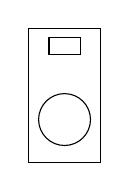
\begin{tikzpicture}[x=0.75pt,y=0.75pt,yscale=-0.5,xscale=0.5]
			\draw   (304,167) .. controls (304,153.19) and (315.19,142) .. (329,142) .. controls (342.81,142) and (354,153.19) .. (354,167) .. controls (354,180.81) and (342.81,192) .. (329,192) .. controls (315.19,192) and (304,180.81) .. (304,167) -- cycle ;
	%Shape: Rectangle [id:dp910627107725476] 
	\draw   (314,88) -- (344,88) -- (344,104) -- (314,104) -- cycle ;
	%Shape: Rectangle [id:dp6936047837352204] 
	\draw   (294,79) -- (364,79) -- (364,208) -- (294,208) -- cycle ;
		\end{tikzpicture}
		\end{center}		
		\\[0.6\textheight]
	\end{tabular}
	% Steps and Scoring	
	\begin{tabular}{ | p{0.65\textwidth} |}
		\hline
		%%%%%%%%%%%%%%%%%%%%%%%%%%%
		% Steps                   %
		%%%%%%%%%%%%%%%%%%%%%%%%%%%
		\rowcolor[HTML]{C0C0C0}Steps\\ 
		\hline
		\tiny \begin{enumerate}[topsep=0pt, partopsep=0pt]
			\item one % EDIT HERE
			\item two
		\end{enumerate}		
		\\ [0.25\textheight]
		\hline
		%%%%%%%%%%%%%%%%%%%%%%%%%%%
		% Scoring                 %
		%%%%%%%%%%%%%%%%%%%%%%%%%%%
		\rowcolor[HTML]{C0C0C0}Scoring \\
		\hline
		\tiny \begin{itemize}[topsep=0pt, partopsep=0pt]
			\item one % EDIT HERE
			\item Passing Hit Factor HF): 
		\end{itemize}		
		\\ [0.25\textheight]
		\hline
	\end{tabular}
\end{document}
